

\tikzset{every picture/.style={line width=0.75pt}} %set default line width to 0.75pt        

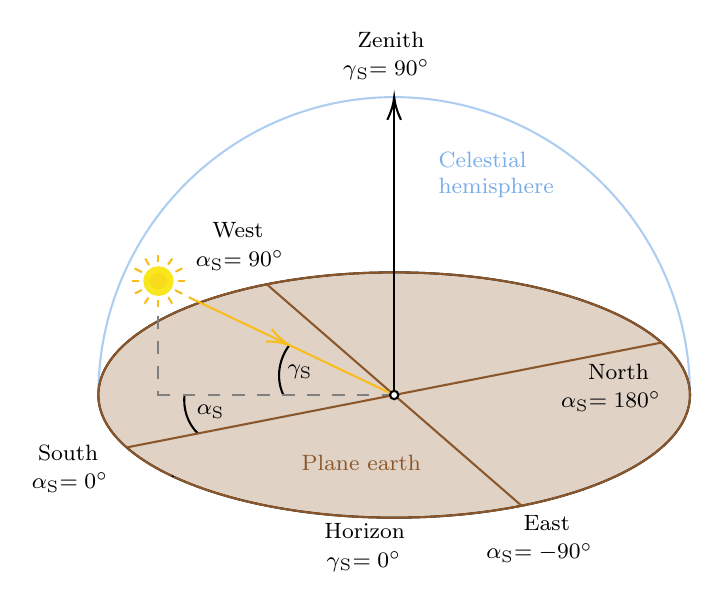
\begin{tikzpicture}[x=0.75pt,y=0.75pt,yscale=-1,xscale=1]
%uncomment if require: \path (0,445); %set diagram left start at 0, and has height of 445






%Shape: Ellipse [id:dp10248886204350427] 
\draw  [color={rgb, 255:red, 0; green, 0; blue, 0 }  ,draw opacity=1 ][fill={rgb, 255:red, 139; green, 87; blue, 42 }  ,fill opacity=0.27 ] (120.55,216.48) .. controls (120.55,183.84) and (184.36,157.39) .. (263.08,157.39) .. controls (341.79,157.39) and (405.61,183.84) .. (405.61,216.48) .. controls (405.61,249.12) and (341.79,275.58) .. (263.08,275.58) .. controls (184.36,275.58) and (120.55,249.12) .. (120.55,216.48) -- cycle ;
%Shape: Arc [id:dp9824695676563142] 
\draw  [draw opacity=0] (120.55,216.48) .. controls (120.55,216.48) and (120.55,216.48) .. (120.55,216.48) .. controls (120.55,137.22) and (184.36,72.96) .. (263.08,72.96) .. controls (341.79,72.96) and (405.61,137.22) .. (405.61,216.48) -- (263.08,216.48) -- cycle ; \draw  [color={rgb, 255:red, 74; green, 144; blue, 226 }  ,draw opacity=0.45 ] (120.55,216.48) .. controls (120.55,216.48) and (120.55,216.48) .. (120.55,216.48) .. controls (120.55,137.22) and (184.36,72.96) .. (263.08,72.96) .. controls (341.79,72.96) and (405.61,137.22) .. (405.61,216.48) ;
%Shape: Ellipse [id:dp6726138734461271] 
\draw  [color={rgb, 255:red, 248; green, 231; blue, 28 }  ,draw opacity=1 ][fill={rgb, 255:red, 248; green, 220; blue, 28 }  ,fill opacity=1 ][line width=2.25]  (143.71,161.61) .. controls (143.71,158.48) and (146.3,155.95) .. (149.5,155.95) .. controls (152.7,155.95) and (155.3,158.48) .. (155.3,161.61) .. controls (155.3,164.73) and (152.7,167.27) .. (149.5,167.27) .. controls (146.3,167.27) and (143.71,164.73) .. (143.71,161.61) -- cycle ;
%Straight Lines [id:da22837958638990763] 
\draw [color={rgb, 255:red, 248; green, 189; blue, 28 }  ,draw opacity=1 ]   (149.5,148.94) -- (149.5,152.47) ;
%Straight Lines [id:da36410436567305116] 
\draw [color={rgb, 255:red, 248; green, 189; blue, 28 }  ,draw opacity=1 ]   (162.47,161.61) -- (158.86,161.61) ;
%Straight Lines [id:da7784535438011968] 
\draw [color={rgb, 255:red, 248; green, 189; blue, 28 }  ,draw opacity=1 ]   (149.5,174.27) -- (149.5,170.75) ;
%Straight Lines [id:da02148874103533327] 
\draw [color={rgb, 255:red, 248; green, 189; blue, 28 }  ,draw opacity=1 ]   (140.14,161.61) -- (136.53,161.61) ;
%Straight Lines [id:da5806655094182651] 
\draw [color={rgb, 255:red, 248; green, 189; blue, 28 }  ,draw opacity=1 ]   (157.5,165.91) -- (160.98,167.72) ;
%Straight Lines [id:da9042107417993022] 
\draw [color={rgb, 255:red, 248; green, 189; blue, 28 }  ,draw opacity=1 ]   (138.03,155.49) -- (141.5,157.31) ;
%Straight Lines [id:da8739850131703888] 
\draw [color={rgb, 255:red, 248; green, 189; blue, 28 }  ,draw opacity=1 ]   (160.98,155.49) -- (157.7,157.08) ;
%Straight Lines [id:da9973855947966144] 
\draw [color={rgb, 255:red, 248; green, 189; blue, 28 }  ,draw opacity=1 ]   (141.5,165.91) -- (138.23,167.49) ;
%Straight Lines [id:da23606504338204548] 
\draw [color={rgb, 255:red, 248; green, 189; blue, 28 }  ,draw opacity=1 ]   (154.14,153.67) -- (156.11,150.74) ;
%Straight Lines [id:da06728456263139648] 
\draw [color={rgb, 255:red, 248; green, 189; blue, 28 }  ,draw opacity=1 ]   (142.78,172.46) -- (144.75,169.53) ;
%Straight Lines [id:da5070173352082208] 
\draw [color={rgb, 255:red, 248; green, 189; blue, 28 }  ,draw opacity=1 ]   (154.26,169.3) -- (156.11,172.47) ;
%Straight Lines [id:da536701929565258] 
\draw [color={rgb, 255:red, 248; green, 189; blue, 28 }  ,draw opacity=1 ]   (143.13,150.74) -- (144.98,153.91) ;
%Straight Lines [id:da1832197332832679] 
\draw [color={rgb, 255:red, 139; green, 87; blue, 42 }  ,draw opacity=1 ]   (324.28,269.67) -- (263.08,216.48) ;
%Straight Lines [id:da35722852927602045] 
\draw [color={rgb, 255:red, 139; green, 87; blue, 42 }  ,draw opacity=1 ]   (263.08,216.48) -- (201.88,163.3) ;
%Shape: Arc [id:dp6576066040432391] 
\draw  [draw opacity=0] (168.58,235.07) .. controls (163.53,230.23) and (161.29,223.2) .. (162.06,216.13) -- (185.16,216.91) -- cycle ; \draw   (168.58,235.07) .. controls (163.53,230.23) and (161.29,223.2) .. (162.06,216.13) ;
%Shape: Arc [id:dp8644885498360859] 
\draw  [draw opacity=0] (209.82,216.7) .. controls (206.04,209.04) and (207.21,199.65) .. (212.57,192.43) -- (231.46,205.17) -- cycle ; \draw   (209.82,216.7) .. controls (206.04,209.04) and (207.21,199.65) .. (212.57,192.43) ;
%Straight Lines [id:da40176543382530383] 
\draw [color={rgb, 255:red, 248; green, 189; blue, 28 }  ,draw opacity=1 ]   (263.08,216.48) -- (212.58,192.42) ;
%Straight Lines [id:da43066607290523007] 
\draw [color={rgb, 255:red, 128; green, 128; blue, 128 }  ,draw opacity=1 ] [dash pattern={on 4.5pt off 4.5pt}]  (149.15,216.48) -- (263.08,216.48) ;
%Straight Lines [id:da9460200323685761] 
\draw [color={rgb, 255:red, 139; green, 87; blue, 42 }  ,draw opacity=1 ]   (133.86,241.81) -- (263.08,216.48) ;
%Straight Lines [id:da12611331746579268] 
\draw [color={rgb, 255:red, 139; green, 87; blue, 42 }  ,draw opacity=1 ]   (263.08,216.48) -- (392.3,191.15) ;
%Shape: Arc [id:dp7682340536128898] 
\draw  [draw opacity=0] (155.96,255.47) .. controls (133.92,245.06) and (120.55,231.42) .. (120.55,216.48) .. controls (120.55,183.84) and (184.36,157.39) .. (263.08,157.39) .. controls (341.79,157.39) and (405.61,183.84) .. (405.61,216.48) .. controls (405.61,249.12) and (341.79,275.58) .. (263.08,275.58) .. controls (220.87,275.58) and (182.95,267.97) .. (156.85,255.88) -- (263.08,216.48) -- cycle ; \draw  [color={rgb, 255:red, 139; green, 87; blue, 42 }  ,draw opacity=1 ] (155.96,255.47) .. controls (133.92,245.06) and (120.55,231.42) .. (120.55,216.48) .. controls (120.55,183.84) and (184.36,157.39) .. (263.08,157.39) .. controls (341.79,157.39) and (405.61,183.84) .. (405.61,216.48) .. controls (405.61,249.12) and (341.79,275.58) .. (263.08,275.58) .. controls (220.87,275.58) and (182.95,267.97) .. (156.85,255.88) ;
%Straight Lines [id:da15722411504245715] 
\draw [color={rgb, 255:red, 128; green, 128; blue, 128 }  ,draw opacity=1 ] [dash pattern={on 4.5pt off 4.5pt}]  (149.5,178.56) -- (149.5,216.93) ;
%Straight Lines [id:da003502427569964439] 
\draw [color={rgb, 255:red, 248; green, 189; blue, 28 }  ,draw opacity=1 ]   (210.77,191.57) -- (164.08,169.36) ;
\draw [shift={(212.57,192.43)}, rotate = 205.44] [color={rgb, 255:red, 248; green, 189; blue, 28 }  ,draw opacity=1 ][line width=0.75]    (10.93,-3.29) .. controls (6.95,-1.4) and (3.31,-0.3) .. (0,0) .. controls (3.31,0.3) and (6.95,1.4) .. (10.93,3.29)   ;
%Straight Lines [id:da8840339574734517] 
\draw    (263.08,216.48) -- (263.08,74.96) ;
\draw [shift={(263.08,72.96)}, rotate = 450] [color={rgb, 255:red, 0; green, 0; blue, 0 }  ][line width=0.75]    (10.93,-3.29) .. controls (6.95,-1.4) and (3.31,-0.3) .. (0,0) .. controls (3.31,0.3) and (6.95,1.4) .. (10.93,3.29)   ;
%Shape: Circle [id:dp5710959149747352] 
\draw  [fill={rgb, 255:red, 255; green, 255; blue, 255 }  ,fill opacity=1 ] (261.08,216.48) .. controls (261.08,215.38) and (261.97,214.48) .. (263.08,214.48) .. controls (264.18,214.48) and (265.08,215.38) .. (265.08,216.48) .. controls (265.08,217.59) and (264.18,218.48) .. (263.08,218.48) .. controls (261.97,218.48) and (261.08,217.59) .. (261.08,216.48) -- cycle ;

% Text Node
\draw (210.29,200.68) node [anchor=north west][inner sep=0.75pt]  [font=\footnotesize]  {$\gamma _{\mathrm{S}}$};
% Text Node
\draw (166.49,219.8) node [anchor=north west][inner sep=0.75pt]  [font=\footnotesize]  {$\alpha _{\mathrm{S}}$};
% Text Node
\draw (217,244) node [anchor=north west][inner sep=0.75pt]  [font=\footnotesize,color={rgb, 255:red, 139; green, 87; blue, 42 }  ,opacity=1 ] [align=left] {Plane earth};
% Text Node
\draw (87,252.4) node [anchor=north west][inner sep=0.75pt]  [font=\footnotesize]  {$\textcolor[rgb]{0,0,0}{\alpha }\textcolor[rgb]{0,0,0}{_{\mathrm{S}}}\textcolor[rgb]{0,0,0}{=0}\textcolor[rgb]{0,0,0}{^{\circ }}$};
% Text Node
\draw (90,239) node [anchor=north west][inner sep=0.75pt]  [font=\footnotesize] [align=left] {South};
% Text Node
\draw (324,273) node [anchor=north west][inner sep=0.75pt]  [font=\footnotesize] [align=left] {East};
% Text Node
\draw (306,286.4) node [anchor=north west][inner sep=0.75pt]  [font=\footnotesize]  {$\textcolor[rgb]{0,0,0}{\alpha }\textcolor[rgb]{0,0,0}{_{\mathrm{S}}}\textcolor[rgb]{0,0,0}{=-90}\textcolor[rgb]{0,0,0}{^{\circ }}$};
% Text Node
\draw (244,40) node [anchor=north west][inner sep=0.75pt]  [font=\footnotesize] [align=left] {Zenith};
% Text Node
\draw (237,53.4) node [anchor=north west][inner sep=0.75pt]  [font=\footnotesize]  {$\textcolor[rgb]{0,0,0}{\gamma }\textcolor[rgb]{0,0,0}{_{\mathrm{S}}}\textcolor[rgb]{0,0,0}{=90}\textcolor[rgb]{0,0,0}{^{\circ }}$};
% Text Node
\draw (174,132) node [anchor=north west][inner sep=0.75pt]  [font=\footnotesize] [align=left] {West};
% Text Node
\draw (166,145.4) node [anchor=north west][inner sep=0.75pt]  [font=\footnotesize]  {$\textcolor[rgb]{0,0,0}{\alpha }\textcolor[rgb]{0,0,0}{_{\mathrm{S}}}\textcolor[rgb]{0,0,0}{=90}\textcolor[rgb]{0,0,0}{^{\circ }}$};
% Text Node
\draw (342,213.4) node [anchor=north west][inner sep=0.75pt]  [font=\footnotesize]  {$\textcolor[rgb]{0,0,0}{\alpha }\textcolor[rgb]{0,0,0}{_{\mathrm{S}}}\textcolor[rgb]{0,0,0}{=180}\textcolor[rgb]{0,0,0}{^{\circ }}$};
% Text Node
\draw (355,200) node [anchor=north west][inner sep=0.75pt]  [font=\footnotesize] [align=left] {North};
% Text Node
\draw (229,290.4) node [anchor=north west][inner sep=0.75pt]  [font=\footnotesize]  {$\textcolor[rgb]{0,0,0}{\gamma }\textcolor[rgb]{0,0,0}{_{\mathrm{S}}}\textcolor[rgb]{0,0,0}{=0}\textcolor[rgb]{0,0,0}{^{\circ }}$};
% Text Node
\draw (228,277) node [anchor=north west][inner sep=0.75pt]  [font=\footnotesize] [align=left] {Horizon};
% Text Node
\draw (283,98) node [anchor=north west][inner sep=0.75pt]  [font=\footnotesize,color={rgb, 255:red, 74; green, 144; blue, 226 }  ,opacity=0.74 ] [align=left] {Celestial\\hemisphere};


\end{tikzpicture}
